\section{Disharta}\label{disharta}

Tags: Stato Creatore: Lorenzo

\section{Disharta}\label{disharta-1}

\begin{center}\rule{0.5\linewidth}{0.5pt}\end{center}

\begin{figure}
\centering
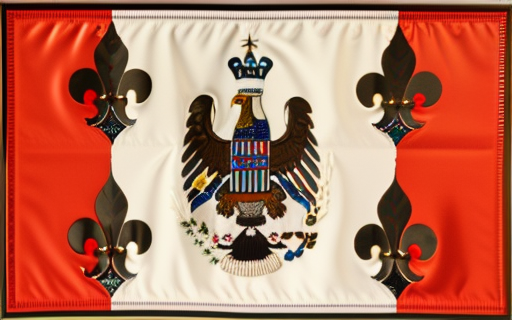
\includegraphics{flag.png}
\caption{flag.png}
\end{figure}

Informazioni Generali

Nome Ufficiale: Impero di Disharta

Lingue Ufficiali: Dishartiano, Valtarese

Capitale: Goldendoor

Forma di Governo: Monarchia Assoluta

Popolazione:

Superficie:

Continente:

Alleati: Gilda dei Commercianti del NordOvest

\begin{center}\rule{0.5\linewidth}{0.5pt}\end{center}

\subsection{1. Descrizione Generale}\label{descrizione-generale}

\begin{center}\rule{0.5\linewidth}{0.5pt}\end{center}

L'Impero di Disharta è un vasto e diversificato impero che si estende su
un territorio immenso, abbracciando una serie di regioni geograficamente
e culturalmente eterogenee. Nella regione Sud-Occidentale dell'impero
sorge la maestosa capitale, Goldendoor, il cui sfavillante splendore è
in netto contrasto con le regioni periferiche più remote. L'Impero è
caratterizzato da una profonda divisione sociale e culturale, con le
diverse comunità che coesistono in un equilibrio teso.

\subsection{2. Storia}\label{storia}

\begin{center}\rule{0.5\linewidth}{0.5pt}\end{center}

L'Impero di Disharta ha una storia intrisa di conquiste militari e
dominazione. È nato dalla crescita dell'influenza di Goldendoor, che ha
gradualmente esteso il proprio dominio su terre lontane. Queste
conquiste hanno spesso incontrato resistenza da parte delle popolazioni
locali, molte delle quali sono ancora riluttanti a sottomettersi al
potere imperiale. Questa storia di conquista e dominio ha lasciato
cicatrici profonde nelle regioni periferiche, alimentando tensioni e
rivendicazioni separatiste.

\subsection{3. Geografia}\label{geografia}

\begin{center}\rule{0.5\linewidth}{0.5pt}\end{center}

\begin{figure}
\centering
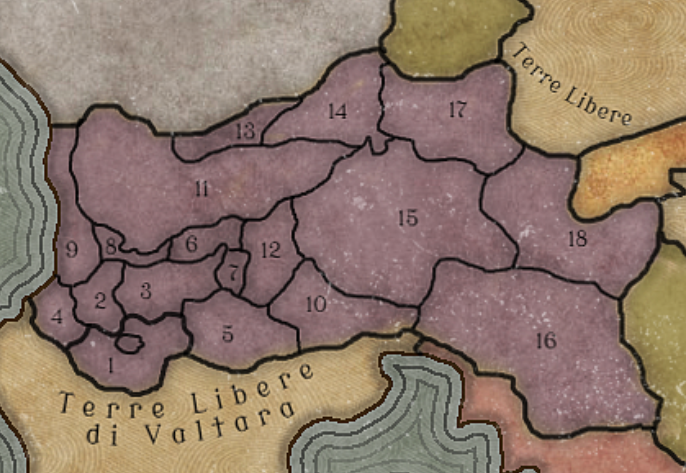
\includegraphics{DISHARTA_PROVINCIE.png}
\caption{DISHARTA\_PROVINCIE.png}
\end{figure}

L'Impero di Disharta è caratterizzato da una vasta e variegata
geografia. Comprende regioni costiere, catene montuose, vaste pianure e
zone desertiche. Le differenze geografiche si riflettono nelle diverse
economie regionali e nelle culture locali. La capitale, Goldendoor,
sorge su una fertile pianura ed è il centro politico ed economico
dell'Impero. Il territorio dell'Impero è diviso amministrativamente in
18 province e 1 distretto:

\begin{itemize}
\tightlist
\item
  Distretto di Goldendoor
\end{itemize}

\begin{enumerate}
\def\labelenumi{\arabic{enumi}.}
\tightlist
\item
  Provincia di Maridona
\item
  Provincia di Cedrelia
\item
  Provincia di Valerantha
\item
  Provincia di Thessamar
\item
  Provincia di Fagot
\item
  Provincia di Lyriandor
\item
  Provincia di Silvershore
\item
  Provincia di Ironspire
\item
  Provincia di Eldergrove
\item
  Provincia del Mitegard Nord-Orientale
\item
  Provincia di Frostholme
\item
  Provincia di Stormwatch
\item
  Provincia di Emberhold
\item
  Provincia di Stonehaven
\item
  Provincia di Sunreach
\item
  Provincia di Windmere
\item
  Provincia di Shadowfen
\item
  Provincia di Ebonhurst
\end{enumerate}

\subsection{4. Demografia}\label{demografia}

\begin{center}\rule{0.5\linewidth}{0.5pt}\end{center}

L'Impero ospita una popolazione diversificata, con una vasta gamma di
gruppi etnici, lingue e tradizioni culturali. Le principali popolazioni
vivono principalmente nelle regioni costiere e nelle pianure
Sud-Occidentali, mentre le regioni periferiche sono abitate da gruppi
più isolati e spesso marginalizzati. Questa diversità demografica è una
delle sfide principali nell'amministrazione e nel mantenimento
dell'unità imperiale.

\subsection{5. Economia}\label{economia}

\begin{center}\rule{0.5\linewidth}{0.5pt}\end{center}

L'economia dell'Impero di Disharta è altamente diversificata. Le regioni
costiere sono caratterizzate dal commercio marittimo e dalla pesca,
mentre le regioni centrali si concentrano sull'agricoltura e
l'allevamento. Tuttavia, la disuguaglianza economica è una
caratteristica distintiva dell'Impero, con le regioni più remote spesso
trascurate e impoverite.

\subsection{6. Cultura}\label{cultura}

\begin{center}\rule{0.5\linewidth}{0.5pt}\end{center}

La cultura dell'Impero di Disharta è eclettica e multiforme, con una
ricca varietà di lingue, religioni, tradizioni culinarie e pratiche
culturali. Questa diversità culturale è spesso una fonte di orgoglio per
molte comunità, ma può anche portare a tensioni e conflitti: la cultura
dominante della capitale è la sua lingua sono imposte come obbligatorie
in tutto l'impero, venendo spesso viste come estranee, e spesso
rifiutate nelle regioni più periferiche. La cultura imperiale è di
origine valtariana: il distretto di Goldendoor e le 3 provincie di
Maridonia, di Fagot e del Mitegard Nord-Orientale fanno parte della
regione storica del Mitegard, o Mitegard Settentrionale, per
distinguerlo dai territori del Mitegard Meridionale facente parte delle
Terre Libere valtariane. La lingua Dishartiana ha un alto grado di
intelligibilità con il Comune Valtarese.

\subsection{7. Governo}\label{governo}

\begin{center}\rule{0.5\linewidth}{0.5pt}\end{center}

L'Impero è una monarchia assoluta, con l'Imperatore al vertice del
potere. L'attuale sovrano è Lucius III, ma il potere centrale è spesso
contestato dalle diverse regioni dell'Impero. Le questioni di autonomia
regionale, lingua e identità culturale sono spesso soppresse dal governo
centrale. Mantenere l'unità imperiale è una delle sfide più grandi per
l'impero, soprattutto negli ultimi decenni, caratterizzati da forti
contrasti.
